\documentclass[tikz,border=6pt]{standalone}
\usetikzlibrary{patterns,arrows.meta,calc}
\begin{document}
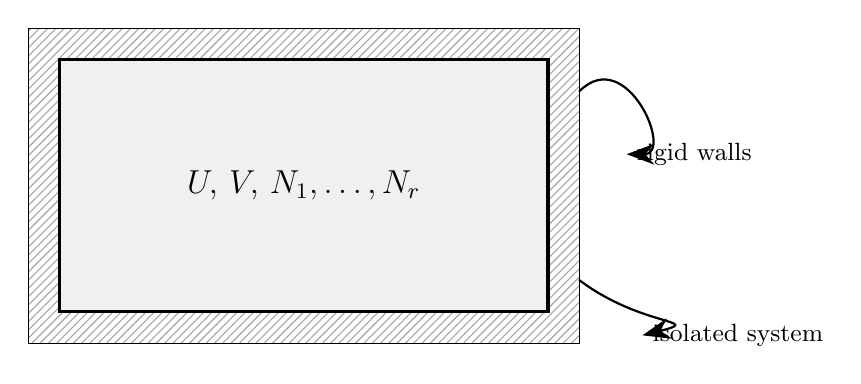
\begin{tikzpicture}[line cap=round]
  % Styles
  \tikzset{
    rigid/.style={pattern=north east lines, pattern color=gray!70},
    wall/.style={line width=1.2pt},
    label/.style={font=\small}
  }

  % Colors
  \colorlet{wallfill}{gray!12}
  \colorlet{rigidclr}{gray!55}

  % Outer rigid shell
  \draw[rigid] (0,0) rectangle (7,4);
  % Inner cavity
  \fill[wallfill] (0.4,0.4) rectangle (6.6,3.6);
  \draw[wall] (0.4,0.4) rectangle (6.6,3.6);

  % Interior text
  \node[font=\large] at (3.5,2.0) {$U,\,V,\,N_1,\ldots,N_r$};

  % Labels with arrows
  \draw[-{Stealth[length=10pt]},thick]
    ($(7,3.2)$) .. controls +(0.6,0.6) and +(0.6,0) .. ($(7.6,2.4)$)
    node[right,label] {rigid walls};

  \draw[-{Stealth[length=10pt]},thick]
    ($(7,0.8)$) .. controls +(0.8,-0.6) and +(0.8,0.2) .. ($(7.8,0.1)$)
    node[right,label] {isolated system};
\end{tikzpicture}
\end{document}
